\section{Desarrollo}

\subsection{Rerequerimientos}

Para este trabajo practico se nos solicita realizar un circuito resonante que cumpla con las siguientes especificaciones:

\begin{itemize}
    \item Frecuencia de resonancia: $f_0 = 16 MHz$
    \item Ancho de banda: $BW = 1.6 MHz$
    \item Factor de calidad con el circuito cargado: $Q_c = 10$
    \item Impedancia de entrada: $Z_{in} = 50 \Omega$
    \item Impedancia de salida: $Z_{out} = 1 k\Omega$
\end{itemize}

\subsection{Diseño del inductor}

El primer paso para construir el circuito resontate es realizar los calculos del inductor. Para ello, se utilizara la siguiente formula:

% L = D^3 * Ns^2 k 10^-3 [micro H]
\begin{equation}
    L = D^3 \cdot N_s^2 \cdot k \cdot 10^{-3}\; [\mu Hy]
\end{equation}

Donde:

\begin{itemize}
    \item $D$ es el diametro externo del inductor en cm 
    \item $N_s$ es el numero de espiras por unidad de longitud en espiras/cm
    \item $k$ es la constante que depende de la relacion de longitud con diametro l/D
\end{itemize}

Para comenzar fijaremos parametros que podamos ajustarlos o determinarlos. Elegimos los siguientes valores:

\begin{itemize}
    \item $D =  2.21\; \text{cm}$
    \item diametro del conductor: $d = 2.1\; \text{mm}$
    \item separacion entre espiras: $S = 3\; \text{mm}$
\end{itemize}

El  \textit{valor del diametro $D$} es el \textit{ diametro interno del inductor $D_o$} mas textit{el diametro del conductor $d$}. El diametro interno del inductor $D_o$ es de 20 mm se eligio por comodidad para el bobinado.
El cilindro para enrrollar el inductor de diametro 20 mm se obtuvo mediante una impresora 3D.


Con estos valores, se puede calcular el \textit{numero de espiras por unidad de longitud $N_s$}:

\begin{equation}
    N_s = \frac{1}{S + d} = \frac{10}{3 + 2.1 } = 1.96 \approx 2 \; \text{espiras/cm}
\end{equation}

Para seguir con los calculos necesitaremos seleccionar un valor de \textit{longitud del inductor $l$}. En la planilla de calculo se definieron valores de longitud con un paso de 0.1 cm, desde 1 cm a 6 cm.
Finalmente seleccionamos:

% separar unidad de numero 
\begin{itemize}
    \item $l = 3.8\; \text{cm}$
\end{itemize}

Calculamos la cantidad de espiras, este valor tiene que ser un numero entero por lo tanto redondeamos:

\begin{equation}
    N = N_s \cdot l = 2 \cdot 3.8 \approx 7\; \text{espiras} 
\end{equation}

Tenemos que tener en cuenta que redondeamos para Ns de 1.96 a 2. Ahora calculamos la \textit{relacion de longitud con diametro}:

\begin{equation}
    \frac{l}{D} = \frac{3.8}{2.21} = 1.72
\end{equation}

Ahora tendremos que calcular la \textit{constante k}, para utilizaremos la formula de Nagaoka. Tambien podemos extraer el valor de la siguiente grafica de la curva de K:

\begin{figure}[H]
    \centering
    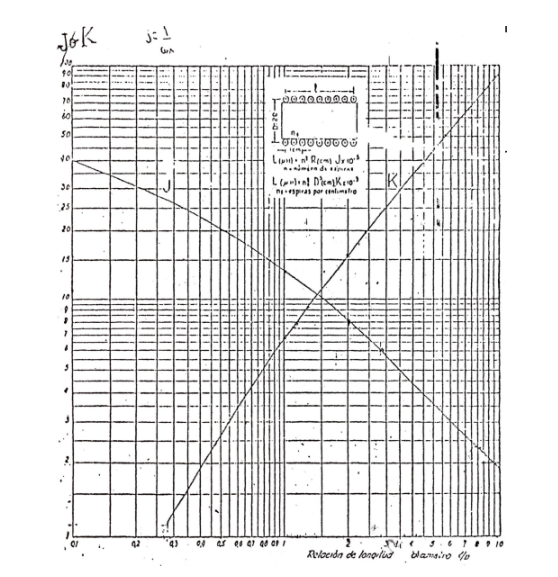
\includegraphics[width=0.5\textwidth]{Imagenes/curva.png}
    \caption{Curva de Nagaoka}
\end{figure}

Nosotros utilizaremos la siguiente formula, que es la funcion de la curva de Nagaoka:

% k = K * Pi ^2 * L/D
\begin{equation}
    k = K \cdot \pi^2 \cdot \frac{L}{D} 
\end{equation}

Donde $K$ se calcula mediante la siguiente formula:

% K = 1 / (1 + 0.9 D/2L - 2*10^-2 (D/2L)^2)
\begin{equation}
    K = \frac{1}{1 + 0.9 \cdot \frac{D}{2L} - 2 \cdot 10^{-2} \left(\frac{D}{2L}\right)^2}
\end{equation}

Sustituyendo los valores obtenemos:

\begin{equation}
    K = \frac{1}{1 + 0.9 \cdot \frac{2.21}{2 \cdot 3.8} - 0.2 \cdot 10^{-2} \left(\frac{2.21}{2 \cdot 3.8}\right)^2} = 0.79
\end{equation}

Y el factor de Nagaoka:

\begin{equation}
    k = 0.79 \cdot \pi^2 \cdot 1.72 = 13.5
\end{equation}


Con todos estos parametros calculados, podemos calcular el valor de la inductancia:

\begin{equation}
    L = D^3 \cdot N_s^2 \cdot k \cdot 10^{-3} = 2.21^3 \cdot (1.96)^2 \cdot 13.5 \cdot 10^{-3} 
\end{equation}

\begin{equation}
    \boxed{L = 0.56\; \mu H}
\end{equation}

\subsubsection{Calculo de resistencias}

Para el calculo de las resistencias necesitaremos calcular el \textit{factor de calidad sin carga $Q_d$}, con la siguiente formula:

\begin{equation}
    Q_d = 8850 \cdot \frac{D \cdot l}{102 \cdot l + 45 \cdot D} \cdot \sqrt{f_0}
\end{equation}

Donde:

\begin{itemize}
    \item $l$ es la longitud del inductor en cm
    \item $D$ es el diametro del inductor en cm
    \item $f_0$ es la frecuencia de resonancia en MHz
\end{itemize}

Sustituyendo los valores obtenemos:

\begin{equation}
    \boxed{Q_d = 610.4}
\end{equation}

La \textit{reactancia del inductor $X_L$} es:

\begin{equation}
    X_L = 2 \cdot \pi \cdot f_0 \cdot L = 2 \cdot \pi \cdot 16 \cdot 10^6 \cdot 0.56 \cdot 10^{-6} \approx 56\; \Omega
\end{equation}

Con $X_L$ y $Q_d$ podemos calcular la \textit{resistencia paralela $R_p$}:

\begin{equation}
    R_p = Q_d \cdot X_L = 610.4 \cdot 56 
\end{equation}

\begin{equation}
    \boxed{R_p = 34.3\; k\Omega}
\end{equation}

Con $Q_C$ y $X_L$ podemos calcular la \textit{resistencia total $R_T$}:

\begin{equation}
    R_T = Q_c \cdot X_L
\end{equation}

\begin{equation}
    \boxed{R_T = 560\; \Omega}
\end{equation}

Con los valores calculados podremos calcular la resistencia de carga reflejada $R_L'$ y la resistencia del generador reflejada $R_g'$, para esto tenemos que despejar $R_L'$ y $R_g'$ de la ecuacion 8:

\begin{equation}
    R_L' // R_P = 2 \cdot R_T 
\end{equation}

\begin{equation}
    R_g' = 2 \cdot R_T 
\end{equation}

Despejando $R_L'$ obtenemos:

\begin{equation}
    R_L' = \frac{2 \cdot R_T \cdot R_P}{R_P - 2 \cdot R_T} 
\end{equation}

Sustituyendo los valores obtenemos:

\begin{equation}
    R_L' = \frac{2 \cdot 560 \cdot 34300}{34300 - 2 \cdot 560} = 1161.8\; \Omega
\end{equation}

\begin{equation}
    \boxed{R_L' = 1161.8\; \Omega}
\end{equation}

Y calculando $R_g'$:

\begin{equation}
    R_g' = 2 \cdot 560
\end{equation}

\begin{equation}
    \boxed{R_g' = 1123\; \Omega}
\end{equation}

% subsection de la subsection de diseño
\subsubsection{Calculo de los capacitores}

Con la \textit{frecuencia de resonancia $f_0 = 16 MHz$} y el valor de la inductancia calculado, podemos calcular el valor de la \textit{capacidad total $C_T$} con la siguiente formula:

\begin{equation}
    C_T = \frac{1}{L \cdot (2 \cdot \pi \cdot f_0)^2} = \frac{1}{0.56 \cdot (2 \cdot \pi \cdot 16 \cdot 10^6)^2} 
\end{equation}

\begin{equation}
    \boxed{C_T = 177\; \text{pF}}
\end{equation}

Con las ecuaciones del sistema de ecuaciones 13, podemos calcular $C_1$, $C_2$, $C_3$ y $C_4$:

\begin{equation}
    C_2 = \frac{C}{2} \cdot \sqrt{\frac{R_g'}{R_g}}
\end{equation}

Entonces $C_1$ sera igual a: 

\begin{equation}
    C_1 = \frac{C_2}{\sqrt{R_g' / R_g - 1}}
\end{equation}

Con $C_4$ y $C_3$ nos queda:

\begin{equation}
    C_4 = \frac{C}{2} \cdot \sqrt{\frac{R_L'}{R_L}}
\end{equation}

\begin{equation}
    C_3 = \frac{C_4}{\sqrt{R_L' / R_L - 1}}
\end{equation}

Remplazando los valores obtenemos:

\begin{equation}
    \boxed{C_1 = 112\; \text{pF}}
\end{equation}

\begin{equation}
    \boxed{C_2 = 420\; \text{pF}}
\end{equation}

\begin{equation}
    \boxed{C_3 = 1225\; \text{pF}}
\end{equation}

\begin{equation}
    \boxed{C_4 = 95\; \text{pF}}
\end{equation}

\newpage
\subsection{Simulacion}

Para comprobar el correcto funcionamiento de nuestro circuito, se realizo una simulacion en LTSpice. A continuacion se muestra el circuito simulado:

\begin{figure}[h]
    \centering
    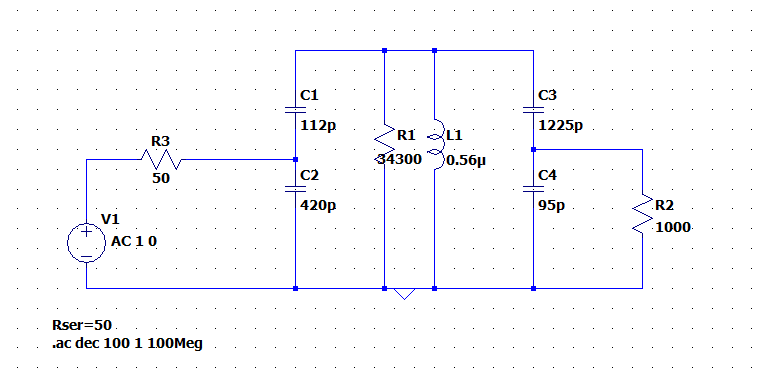
\includegraphics[width=0.7\textwidth]{Imagenes/circuito.png}
    \caption{Circuito simulado en LTSpice}
\end{figure}

La respuesta en frecuencia obtenida del circuito simulada es la siguiente:

\begin{figure}[h]
    \centering
    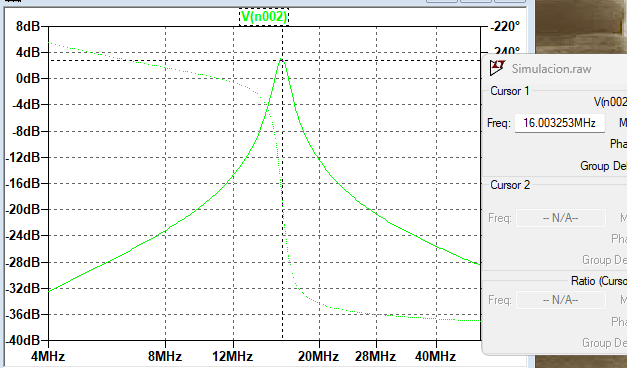
\includegraphics[width=0.7\textwidth]{Imagenes/resultado_circuito.png}
    \caption{Respuesta en frecuencia del circuito simulado}
\end{figure}

Se observa que la \textit{frecuencia de resonancia es de $16 MHz$} con una ganancia de $2 dB$. Ademas:

\begin{itemize}
    \item frecuencia de corte inferior: $15.2 MHz$
    \item frecuencia de corte superior: $16.8 MHz$
    \item ancho de banda: $1.6 MHz$
    \item $Q_c = 10$
\end{itemize}

\newpage
\subsection{Seleccion de componentes y armado}

El primer paso sera determinar que capacitores utilizaremos para el circuito. Los capacitores seleccionados son:

\begin{itemize}
    \item $C_1 = 100\; \text{pF}$
    \item $C_2 = 330 + 100 = 430\; \text{pF}$
    \item $C_3 = 1000 + 100 + 100 =1200\; \text{pF}$
    \item $C_4 = 100\; \text{pF}$
\end{itemize}

La capacidad total sera:

\begin{equation}
    C_T = \frac{C_1 \cdot C_2}{C_1 + C_2} + \frac{C_3 \cdot C_4}{C_3 + C_4} 
\end{equation}


\begin{equation}
    \boxed{C_T = 173.4 \; \text{pF}}
\end{equation}

El resultado obtenido con los capacitores obtenidos, haciendo un analisis de montecarlo:

\begin{figure}[h]
    \centering
    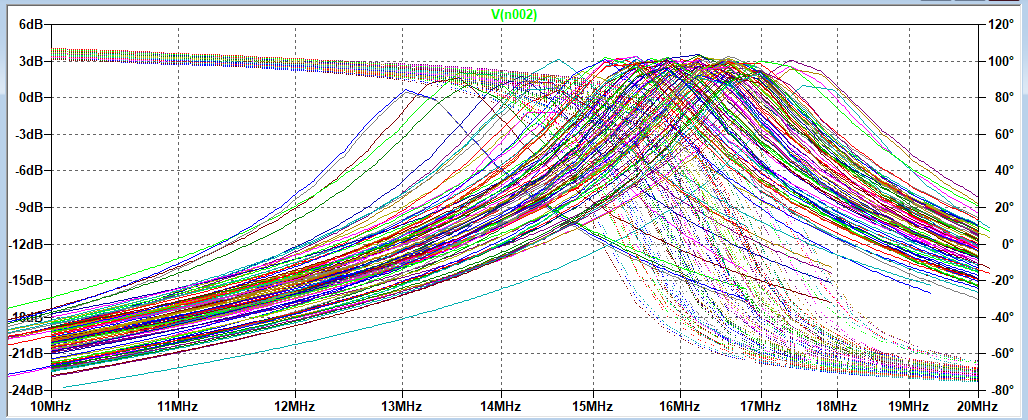
\includegraphics[width=0.7\textwidth]{Imagenes/montecarlo.png}
    \caption{Analisis de montecarlo}
\end{figure}

Vemos que la tolerancia y los capacitores utilizados hace que $f_0$ varie entre $13 MHz$ y $17.2 MHz$.


El inductor y los capacitores montados en la PCB finalmente nos queda:

\begin{figure}[h]
    \centering
    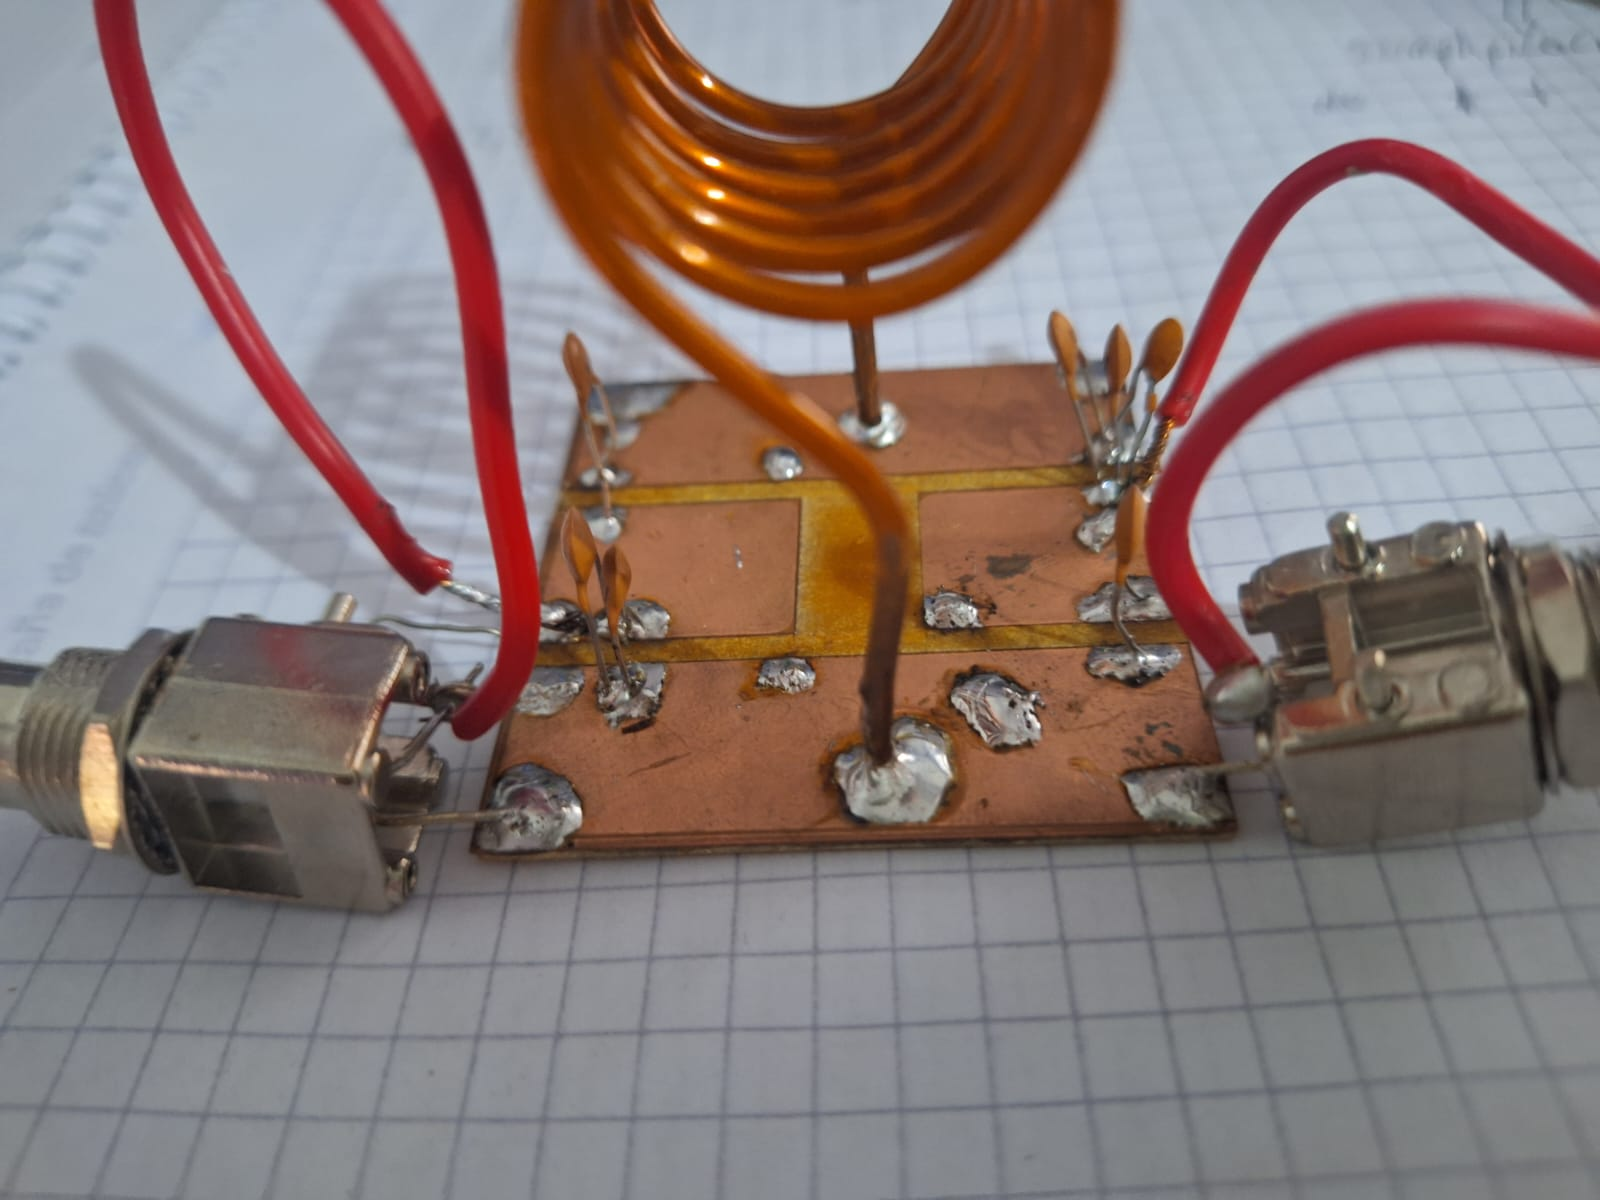
\includegraphics[width=0.7\textwidth]{Imagenes/pcb1.jpeg}
    \caption{PCB montada}
\end{figure}

\begin{figure}[h]
    \centering
    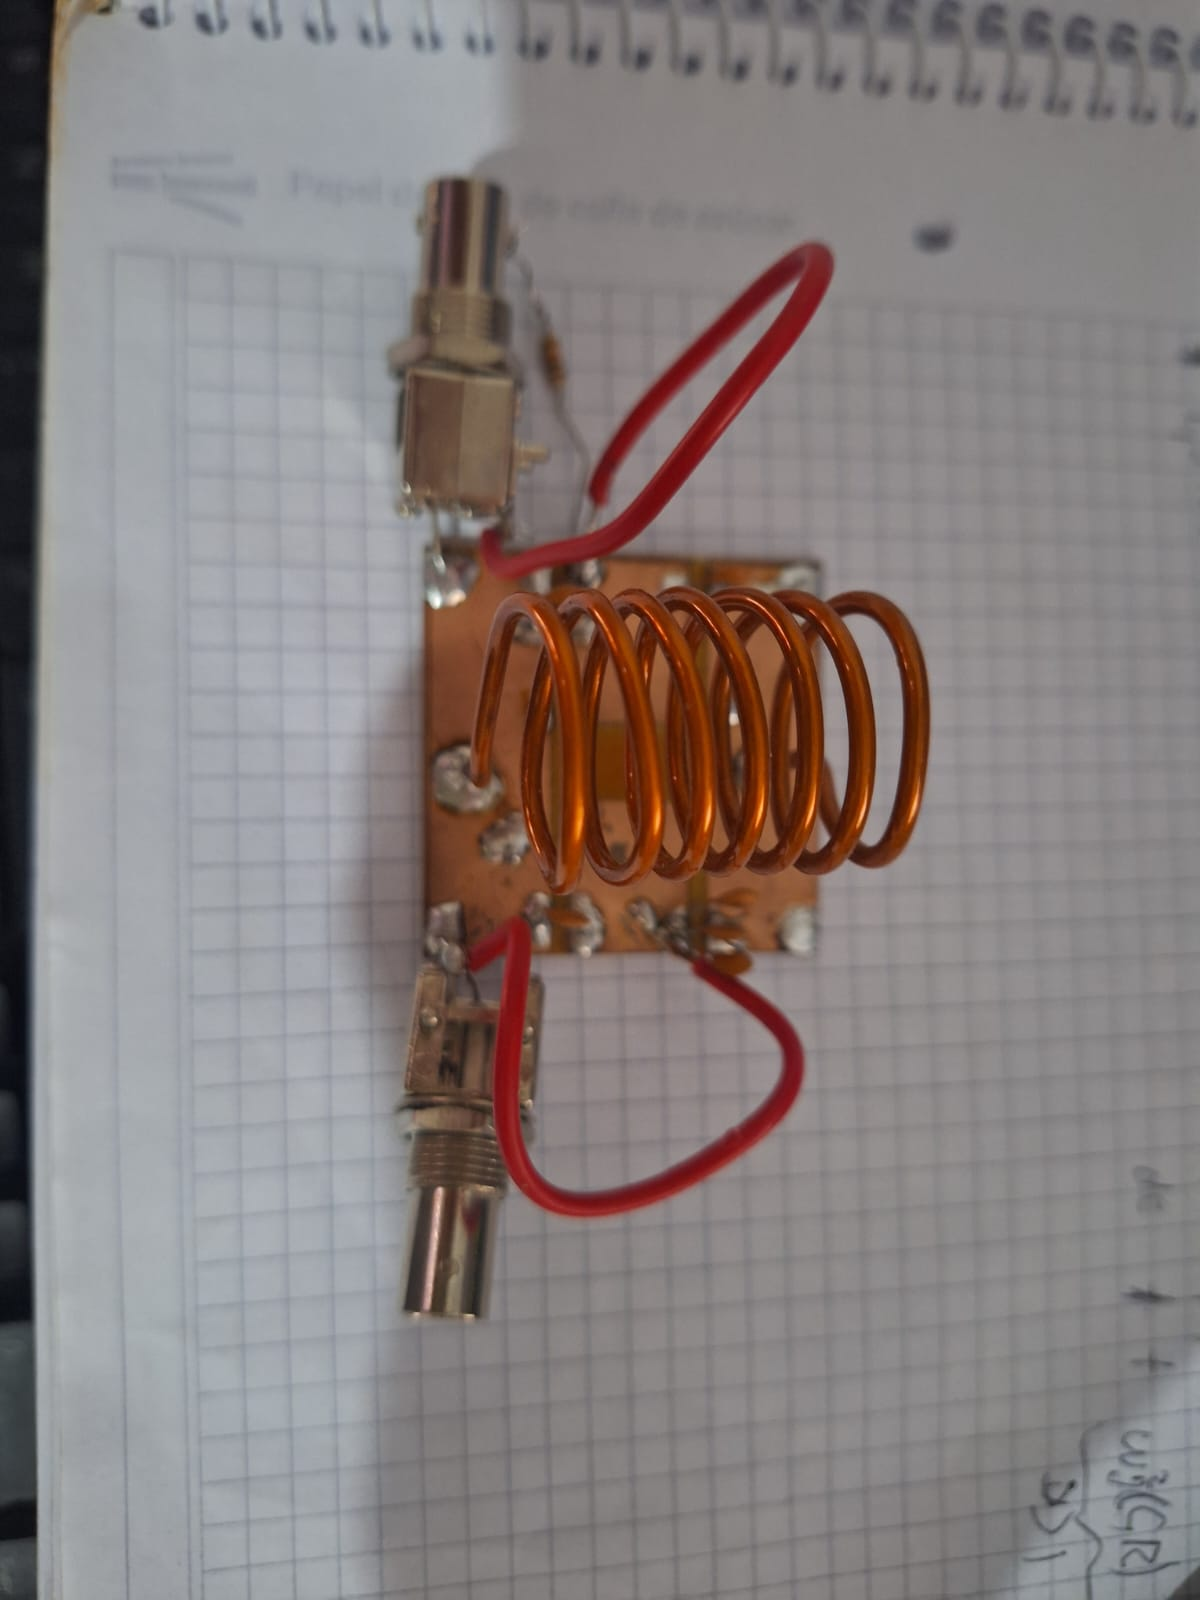
\includegraphics[width=0.7\textwidth]{Imagenes/pcb2.jpeg}
    \caption{PCB montada}
\end{figure}


\newpage
\subsection{Mediciones}

Para la medicion de los parametros del circuito, se utilizara:

\begin{itemize}
    \item Generador de señales
    \item Osciloscopio
    \item 3 cables BNC
    \item BNC-T 
\end{itemize}

El numero de serie de los instrumentos utilizados son:

\begin{itemize}
    \item Generador de señales: GW Instek AFG-2125 (GFA2)
    \item Osciloscopio: Keysight DSO1052B (OSC63)
\end{itemize}

\subsubsection{Medicion de $f_o$}

Para la medicion de la frecuencia de resonancia, se conecta el circuito a tope. El esquema es el siguiente:

\begin{figure}[H]
    \centering
    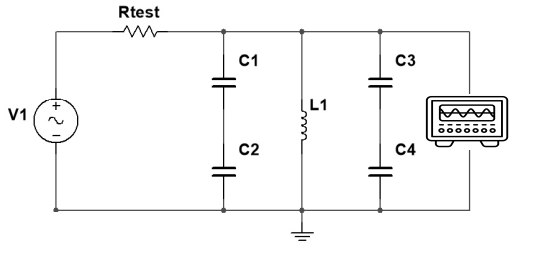
\includegraphics[width=0.5\textwidth]{Imagenes/medicion_fo.png}
    \caption{Medicion de $f_{o1}$}

\end{figure}


La resistencia Rtest tiene que ser del orden de  $R_p$, por lo tanto, inicialmente se utilizó una resistencia de 1 k$\Omega$. Una vez realizada la conexión, se varía la frecuencia del generador 
de señales de menor a mayor hasta encontrar la frecuencia de resonancia. Debemos considerar que el osciloscopio tiene una capacidad de entrada, por lo tanto, esta capacidad parásita puede 
afectar la medición de la frecuencia de resonancia.

La medicion $f_o1$:

\begin{equation}
    \boxed{f_{o1} = 12 MHz}
\end{equation}

A continuacion mediremos la frecuencia de resonancia $f_{o2}$, para esto se utilizara una resistencia de 1k$\Omega$ y ademas, se agrega el capacitor $C_F$ en paralelo al inductor y los capacitores.
El esquema es el siguiente:

\begin{figure}[H]
    \centering
    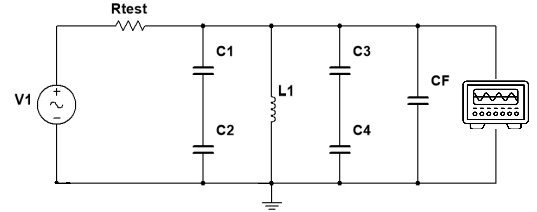
\includegraphics[width=0.5\textwidth]{Imagenes/medicion_fo2.png}
    \caption{Medicion de $f_o2$}
\end{figure}

Donde el capacitor $C_F$ es de 100pF.

La medicion $f_{o2}$:

\begin{equation}
    \boxed{f_o2 = 10.5\; MHz}
\end{equation}

Para obtener la frecuencia de resonancia $f_o$ se debe obtener $C_o$ a partir de estas ecuaciones:

\begin{equation}
    f_{o1} = \frac{1}{2\pi\sqrt{L(C_T + C_o)}}
\end{equation}

\begin{equation}
    f_{o2} = \frac{1}{2\pi\sqrt{L(C_T + C_o + C_F)}}
\end{equation}

Donde $C_T$ es igual a 177 pF. Despejando $C_o$ de estas ecuaciones obtenemos:

\begin{equation}
    \left(\frac{f_{o1}}{f_{o2}}\right)^2 = \frac{C_T + C_o + C_F}{C_T + C_o}
\end{equation}

\begin{equation}
    C_o = \frac{C_T \cdot (f_{o2}^2 - f_{o1}^2) + C_F f_{o2}^2}{f_{o1}^2 - f_{o2}^2}
\end{equation}

El capacitor $C_F$ es de 100 pF y $C_o$ es de:

\begin{equation}
    \boxed{C_o = 149.7\; pF}
\end{equation}

Con este valor, dimensionamos la capacidad agregada del osciloscopio, cables BNC, soldaduras, etc., y es comparable a la del 
circuito, por lo tanto, modificará la medición y afectará el resultado. Ahora determinaremos el valor de la inductancia $L$:

\begin{equation}
    L = \frac{1}{(2\pi f_{o1})^2} \cdot \frac{1}{C_T + C_o}
\end{equation}

\begin{equation}
    \boxed{L = 0.538\; \mu Hy}
\end{equation}

Con este valor determinamos el valor de la \textit{frecuencia de resonancia $f_o$}:

\begin{equation}
    f_o = \frac{1}{2\pi\sqrt{L \cdot C_T}}
\end{equation}

\begin{equation}
    \boxed{f_o = 16.3\; MHz}
\end{equation}


\subsubsection{Medición de $R_p$}

Para la medición de la resistencia de pérdida, se utiliza el esquema de la figura \ref{fig: de la medición de la resistencia de pérdida}:

\begin{figure}[H]
    \centering
    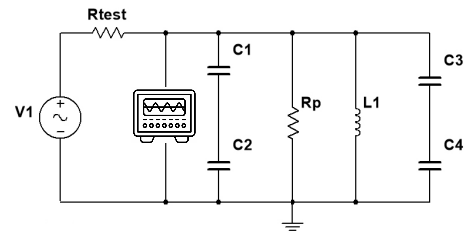
\includegraphics[width=0.8\textwidth]{Imagenes/medicion_rp.png}
    \caption{Medición de $R_p$}
    \label{fig: de la medición de la resistencia de pérdida}
\end{figure}

Tenemos que colocar la frecuencia del generador de onda en la frecuencia de resonancia $f_o$, ya que la reactancia inductiva y capacitiva se anulan.
Por lo tanto, nos quedará la resistencia de test $R_{test} = 1k\Omega$ en serie con la resistencia de pérdida $R_p$. Por lo tanto, realizando el divisor resistivo:

\begin{equation}
    V_{osciloscopio} = V_{1} \cdot \frac{R_p}{R_p + (R_{test}+ R_g)}
\end{equation}

Y despejando $R_p$ obtenemos:

\begin{equation}
    R_p = \frac{(R_{test} + R_g) \cdot V_{osciloscopio}}{V_{1} - V_{osciloscopio}}
\end{equation}

Las mediciones son las siguientes:


% tabla con mediciones de Vosciloscopio y V1

\begin{table}[H]
    \centering
    \begin{tabular}{|c|c|}
    \hline
    \rowcolor[HTML]{C0C0C0} 
    \textbf{Medición} & \textbf{Valor} \\ \hline
    $V_{osciloscopio}$            & 2 V         \\ \hline
    $V_{1}$         & 1.76 V         \\ \hline
    \end{tabular}
\end{table}

Reemplazando los valores obtenemos:

\begin{equation}
    \boxed{R_p = 7.7\; k\Omega}
\end{equation}

Idealmente, la resistencia de pérdida debería ser infinita, o lo suficientemente alta para disminuir la pérdida de energía en el circuito. Además, nosotros hicimos la adaptación
de impedancia suponiendo que:

\begin{equation}
    R_p \parallel R_L = 2 \cdot R_T
\end{equation}

Y el cálculo de este valor tendría que ser de 34.3 k$\Omega$. Por lo tanto, este valor modificará la adaptación de impedancia. 

\subsubsection{Medición de $BW$}

Para la medición del ancho de banda, se utiliza el esquema de la figura \ref{fig: de la medición del ancho de banda}:

% Colocar imagen abajo del texto de arriba
\begin{figure}[h]
    \centering
    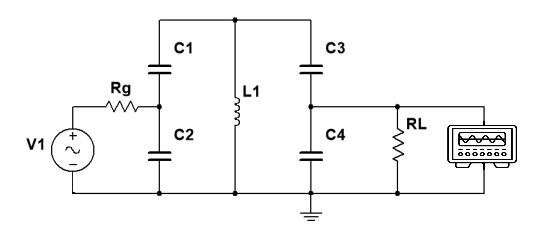
\includegraphics[width=0.5\textwidth]{Imagenes/medicion_bw.png}
    \caption{Medición de $BW$}
    \label{fig: de la medición del ancho de banda}
\end{figure}

La medición del ancho de banda variaremos la frecuencia hasta encontrar el pico máximo de amplitud en la salida, una vez encontrado
el pico máximo, buscaremos -3 dB de la amplitud máxima. La diferencia entre la frecuencia de corte superior y la inferior nos dará el ancho de banda. 
Las mediciones son las siguientes:

% tabla con 3 columnas y 4 filas, frecuencia de corte inferior central y corte superior. Amplitud y frecuencia
\begin{table}[h]
    \centering
    \begin{tabular}{|c|c|c|}
    \hline
    \rowcolor[HTML]{C0C0C0} 
    \textbf{Medición} & \textbf{Amplitud} & \textbf{Ancho de banda} \\ \hline
    Frecuencia de corte inferior            & 2.87 V             & 11.85 MHz                \\ \hline
    Frecuencia central         & 4.06 V             & 12.6 MHz                \\ \hline
    Frecuencia de corte superior            & 2.87 V             & 13.3 MHz                \\ \hline
    \end{tabular}
\end{table}

El ancho de banda es:

\begin{equation}
    BW = f_{corte\; superior} - f_{corte\; inferior} = 13.3 - 11.85
\end{equation}

\begin{equation}
    \boxed{BW = 1.45\; MHz}
\end{equation}

El valor obtenido es menor al esperado, esto puede ser debido a la capacidad parásita del osciloscopio, cables BNC, soldaduras, etc. Además, es posible
que debido a la tolerancia de los componentes y la resistencia de pérdida menor a la calculada, el ancho de banda se vea afectado.

\subsubsection{Medición de $Z_{in}$}

Para la medición de la impedancia de entrada, se utiliza el esquema de la figura \ref{fig: de la medición de la impedancia de entrada}
y la figura \ref{fig: de la medición de la impedancia de entrada 2}:

\begin{figure}[h]
    \centering
    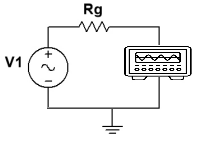
\includegraphics[width=0.5\textwidth]{Imagenes/medicion_zin1.png}
    \caption{Medición de $V_g$}
    \label{fig: de la medición de la impedancia de entrada}
\end{figure}

\newpage

\begin{figure}[h]
    \centering
    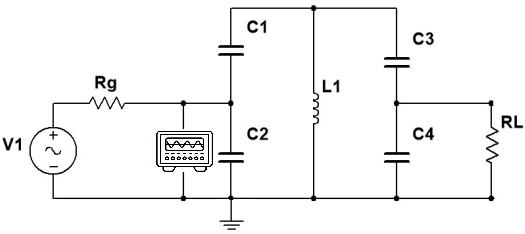
\includegraphics[width=0.8\textwidth]{Imagenes/medicion_zin2.png}
    \caption{Medición de $V_{in}$}
    \label{fig: de la medición de la impedancia de entrada 2}
\end{figure}

Con estas dos mediciones podemos calcular la impedancia de entrada. Las mediciones son las siguientes:
% Tabla con mediciones de Vg y Vin
\begin{table}[H]
    \centering
    \begin{tabular}{|c|c|}
    \hline
    \rowcolor[HTML]{C0C0C0} 
    \textbf{Medición} & \textbf{Valor} \\ \hline
    Generador $V_1$            & 2.3  V         \\ \hline
    Tensión de entrada $V_{in}$         & 0.7 V         \\ \hline
    \end{tabular}
\end{table}

Debido a que medimos en resonancia, la reactancia inductiva y capacitiva se anulan. Por lo tanto, podemos plantear el divisor resistivo:

\begin{equation}
    V_{in} = V_1 \cdot \frac{Z_{in}}{Z_{in} + R_{g}}
\end{equation}

Despejando $Z_{in}$ obtenemos:

\begin{equation}
    Z_{in} = R_g \cdot \frac{ V_{in}}{V_1 - V_{in}}
\end{equation}

Reemplazando los valores obtenemos:

\begin{equation}
    \boxed{Z_{in} = 22\; \Omega}
\end{equation}

Este valor discrepa de forma significativa con el valor esperado de 50 $\Omega$. Esto puede ser debido a la capacidad parásita del osciloscopio, cables BNC, soldaduras, etc. 
La mejor forma de medir la impedancia de entrada es con un analizador de impedancia o con un roímetro. 
Además, una causa que afecta a la impedancia de entrada es la resistencia de pérdida, que en este caso es menor a la calculada.

\subsubsection{Medición de $Z_{out}$}

Para la medición de la impedancia de salida, se utiliza el esquema de la figura \ref{fig: Primer esquema de la medición de la impedancia de salida} y la figura
\ref{fig: Segundo esquema de la medición de la impedancia de salida}.

%
\begin{figure}[h]
    \centering
    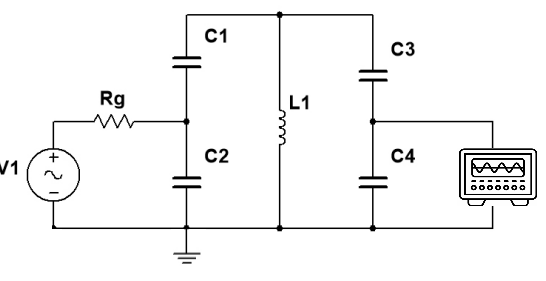
\includegraphics[width=0.8\textwidth]{Imagenes/medicion_zout1.png}
    \caption{Medición de $V_{out}$ sin carga}
    \label{fig: Primer esquema de la medición de la impedancia de salida}
\end{figure}

% 
\begin{figure}[h]
    \centering
    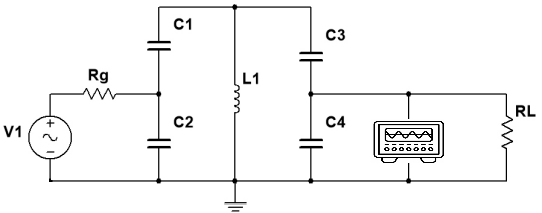
\includegraphics[width=0.8\textwidth]{Imagenes/medicion_zout2.png}
    \caption{Medición de $V_{out}$ con carga}
    \label{fig: Segundo esquema de la medición de la impedancia de salida}
\end{figure}




Realizando estas dos mediciones podemos calcular la impedancia de salida. Las mediciones son las siguientes:

% Tabla con mediciones de Vout sin carga y con carga
\begin{table}[h]
    \centering
    \begin{tabular}{|c|c|}
    \hline
    \rowcolor[HTML]{C0C0C0} 
    \textbf{Medición} & \textbf{Valor} \\ \hline
    $V_{out}$ sin carga            & 1.05  V         \\ \hline
    $V_{out}$ o $V_{L}$ con carga         & 2.4 V         \\ \hline
    \end{tabular}
\end{table}

Planteando el divisor resistivo:

\begin{equation}
    V_{L} = V_{out} \cdot \frac{Z_{L}}{Z_{out} + Z_L}
\end{equation}

Despejando $Z_{out}$ obtenemos:

\begin{equation}
    Z_{out} = Z_L \cdot \frac{V_{out} - V_L}{V_L}
\end{equation}

Reemplazando los valores obtenemos:

\begin{equation}
    \boxed{Z_{out} = 1285\; \Omega}
\end{equation}

El valor difiere del valor esperado de 1 k$\Omega$. Si bien el osciloscopio y los cables pueden modificar la medición, la principal causa de la diferencia es la resistencia de pérdida
que es menor a la calculada. En la siguiente fórmula podemos ver cómo afecta la resistencia de pérdida a la adaptación de impedancia:

\begin{equation}
    R_L' = \frac{2 \cdot R_T}{1 - \frac{2 \cdot R_T}{R_p}}
\end{equation}

Donde podemos observar que si $R_p$ es menor, el término $\frac{2 \cdot R_T}{R_p}$ será considerable y afectará directamente la adaptación de impedancia. 

\subsubsection{Factor de calidad}

Con los valores medidos podemos calcular el \textit{factor de calidad $Q_c$} y el \textit{factor de calidad sin carga $Q_d$}:

\begin{equation}
    Q_c = \frac{f_o}{BW} = \frac{16.3}{1.45}
\end{equation}

\begin{equation}
    \boxed{Q_c = 11.2}
\end{equation}

\begin{equation}
    Q_d = \frac{R_p}{X_L} = \frac{R_p}{2 \cdot \pi \cdot f_o \cdot L} = \frac{7.7 \cdot 10^3}{2 \cdot \pi \cdot 16.3 \cdot 10^6 \cdot 0.538 \cdot 10^{-6}}
\end{equation}

\begin{equation}
    \boxed{Q_d = 139.7}
\end{equation}



